
\section{Architecture Integration}

\subsection{Model Support}

\begin{table}[H]
\centering
\small
\begin{tabular}{llllllll}
\toprule
\textbf{Model} & \textbf{Layers} & \textbf{$d$} & \textbf{$H$} & \textbf{$H_{kv}$} & \textbf{Nested?} & \textbf{Conv1D?} & \textbf{RoPE?} \\
\midrule
DistilBERT-base & 6 & 768 & 12 & 12 & No & No & \textbf{Added} \\
RoBERTa-base & 12 & 768 & 12 & 12 & Yes & No & \textbf{Added} \\
GPT-2 & 12 & 768 & 12 & 12 & No & Yes & \textbf{Added} \\
Qwen3.5-0.8B & 24 & 1024 & 8 & 2 & No & No & Native \\
\bottomrule
\end{tabular}
\end{table}

\textbf{Note.} DistilBERT, RoBERTa, and GPT-2 use absolute position embeddings. 
UnifiedRoPE \textbf{adds} RoPE on top, which may not match pretrained behavior.

For Qwen, RoPE is native -- UnifiedRoPE simply preserves it.

\subsection{DistilBERT (Flat)}

\begin{lstlisting}
distilbert.transformer.layer.0.attention
+-- q\_lin  (Linear 768 $\to$ 768)
+-- k\_lin  (Linear 768 $\to$ 768)
+-- v\_lin  (Linear 768 $\to$ 768)
+-- out\_lin (Linear 768 $\to$ 768)
\end{lstlisting}

\textbf{Weight extraction:}
\begin{lstlisting}
w\_q = src.q\_lin.weight.detach()
w\_k = src.k\_lin.weight.detach()
w\_v = src.v\_lin.weight.detach()
w\_o = src.out\_lin.weight.detach()
\end{lstlisting}

\texttt{is\_nested\_encoder = False}.

\textbf{RoPE caveat.} DistilBERT was trained with absolute positions. Adding 
RoPE changes the attention pattern. Accuracy may drop unless recovery 
fine-tuning adapts.

\subsection{RoBERTa (Nested)}

\begin{lstlisting}
roberta.encoder.layer.0.attention
+-- self
|   +-- query, key, value
+-- output
    +-- dense
\end{lstlisting}

\textbf{Nested detection:}
\begin{lstlisting}
if hasattr(old\_attn, "self") and hasattr(old\_attn, "output"):
    self.is\_nested\_encoder = True
    src = old\_attn.self
    w\_o = old\_attn.output.dense.weight
\end{lstlisting}

\texttt{is\_nested\_encoder = True}. Forward returns raw context.

\subsection{GPT-2 (Causal Conv1D)}

\begin{lstlisting}
transformer.h.0.attn
+-- c\_attn  (Conv1D 768 $\to$ 2304)
+-- c\_proj  (Conv1D 768 $\to$ 768)
\end{lstlisting}

\textbf{Split c\_attn:}
\begin{lstlisting}
c\_attn\_w = src.c\_attn.weight.detach()
if c\_attn\_w.shape[0] == self.hidden\_size and c\_attn\_w.shape[1] != self.hidden\_size:
    c\_attn\_w = c\_attn\_w.t()
q\_dim = self.q\_head\_size
k\_dim = self.kv\_head\_size
v\_dim = self.kv\_head\_size
w\_q = c\_attn\_w[:q\_dim, :]
w\_k = c\_attn\_w[q\_dim:q\_dim+k\_dim, :]
w\_v = c\_attn\_w[q\_dim+k\_dim:, :]
\end{lstlisting}

\texttt{is\_nested\_encoder = False}. Causal mask applied in forward.

\subsection{Qwen3.5 (GQA + RoPE)}

\begin{lstlisting}
model.layers.0.self\_attn
+-- q\_proj  (Linear 1024 $\to$ 2048)
+-- k\_proj  (Linear 1024 $\to$ 512)
+-- v\_proj  (Linear 1024 $\to$ 512)
+-- o\_proj  (Linear 2048 $\to$ 1024)
\end{lstlisting}

\textbf{GQA expansion:}
\begin{lstlisting}
if self.num\_kv\_heads != self.num\_heads:
    k = repeat\_kv(k, self.num\_key\_value\_groups)
    v = repeat\_kv(v, self.num\_key\_value\_groups)
\end{lstlisting}

\textbf{RoPE:} Either internal \texttt{\_apply\_rope} or external \texttt{position\_embeddings}.

\texttt{is\_nested\_encoder = False}.

\subsection{Injection Hook}

\begin{lstlisting}
def inject\_unified\_rope(layer, model\_config=None, comp\_config=None,
                        old\_attn=None, **kwargs):
    src = old\_attn
    if src is None:
        for attr in ("attention", "self\_attn", "attn", "self"):
            if hasattr(layer, attr):
                src = getattr(layer, attr)
                break
    
    if model\_config is None and hasattr(layer, "config"):
        model\_config = layer.config
    
    lora\_rank = kwargs.pop("lora\_rank", 16)
    rank = kwargs.pop("rank", 32)
    
    new\_attn = UnifiedRoPE(
        config=model\_config, rank=rank, lora\_rank=lora\_rank,
        pretrained\_attn=src, **kwargs,
    )
    
    # Replace
    for attr in ("self\_attn", "attn", "self"):
        if hasattr(layer, attr):
            setattr(layer, attr, new\_attn)
            return new\_attn
    if hasattr(layer, "attention"):
        if hasattr(layer.attention, "self"):
            layer.attention.self = new\_attn
        else:
            layer.attention = new\_attn
        return new\_attn
    layer.attention = new\_attn
    return new\_attn
\end{lstlisting}

\textbf{Safe injection.} Wraps in try/except. Logs errors. \textbf{Raises} 
\texttt{RuntimeError} on failure (does not silently return None).

\subsection{Failure Modes}

\begin{table}[H]
\centering
\small
\begin{tabular}{lll}
\toprule
\textbf{Failure} & \textbf{Detection} & \textbf{Response} \\
\midrule
Missing weights & Validation & Raise RuntimeError \\
Near-zero Frobenius & Norm check \textless{} 1e-4 & Raise RuntimeError \\
Cross-attention & Not supported & Not implemented \\
Conv1D wrong orientation & Shape check & Transpose \\
\bottomrule
\end{tabular}
\end{table}

\subsection{Registry}

\begin{lstlisting}
@ATTENTION\_REGISTRY.register("compression\_unified\_rope")
@ATTENTION\_REGISTRY.register("unified\_rope")
@ATTENTION\_REGISTRY.register("unified\_rope\_attention")
class UnifiedRoPE(BaseAttention):
    ...

@ATTENTION\_REGISTRY.register("unified\_rope\_inject")
@ATTENTION\_REGISTRY.register("compression\_unified\_rope\_inject")
@ATTENTION\_REGISTRY.register("inject\_unified\_rope")
def inject\_unified\_rope(...):
    ...
\end{lstlisting}

\subsection{LoRA Recovery Integration}

UnifiedRoPE uses \texttt{LoRALinear} projections with \texttt{freeze\_base=True}. Base 
weights are frozen; only LoRA adapters trained during recovery.

\subsection{Comparison with Companion Methods}

\begin{table}[H]
\centering
\small
\begin{tabular}{lll}
\toprule
\textbf{Method} & \textbf{Type} & \textbf{Purpose} \\
\midrule
MinimalSVD & Compression & Reduce params \\
Dobi-SVD & Compression & Reduce params \\
MLA & Compression & Reduce KV \\
Nystr mformer & Compute & Reduce compute \\
\textbf{UnifiedRoPE} & \textbf{Replacement} & \textbf{Portability} \\
\bottomrule
\end{tabular}
\end{table}

\textbf{UnifiedRoPE is orthogonal} to all compression methods.
\begin{lstlisting}

---
\end{lstlisting}

\begin{figure}[H]
\centering
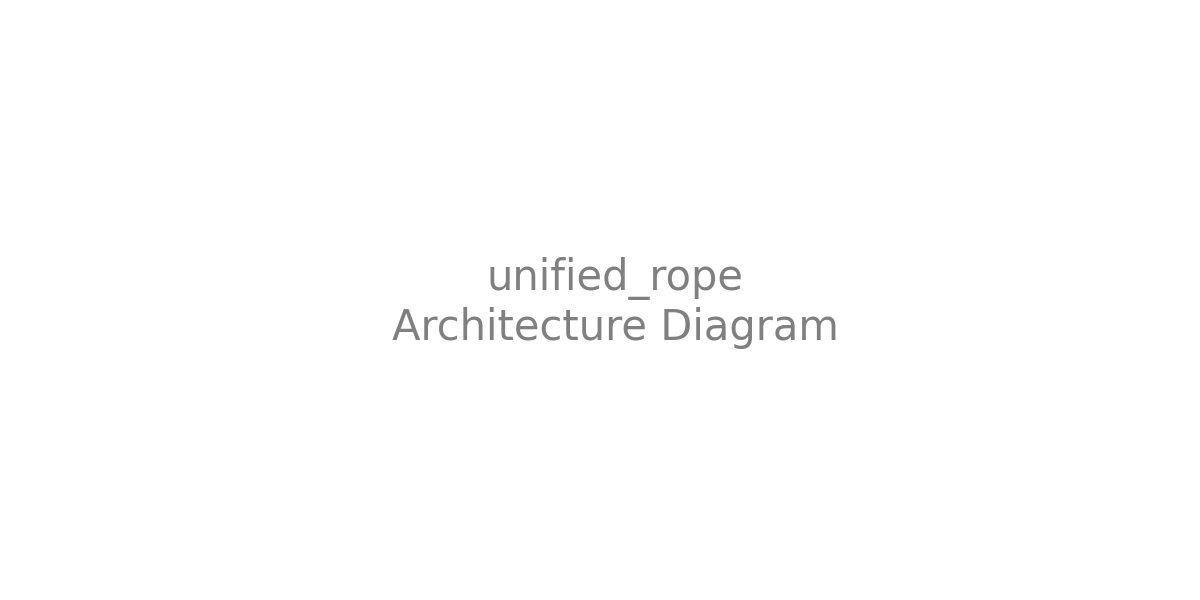
\includegraphics[width=\linewidth]{figures/architecture.png}
\caption{High-level architectural diagram of unified\_rope.}
\label{fig:arch_unified-rope}
\end{figure}

